\section{Penelitian dan Riset Terkait}
Berikut adalah beberapa penelitian dan riset yang pernah dilakukan sebelumnya dan berhubungan dengan tugas akhir ini.

\subsection{\textit{Deep Learning-Based Autoscaling Using Bidirectional Long Short-Term Memory for Kubernetes}}
Riset ini dilakukan oleh Nhat Minh, Dang Quang dan Myungsik Yoo dari \textit{Department of Information Communication Convergence Technology, Soongsil University}, Seoul, Korea Selatan yang dipublikasikan 23 April 2021. Riset ini melakukan pengembangan \textit{autoscaling} menggunakan \textit{deep learning} dengan \textit{Bidirectional Long Short-Term Memory} (Bi-LSTM) untuk melakukan \textit{autoscale} untuk \textit{web server} dengan memperhatikan metrik penggunaan prosesor dan memori.

Menurut riset ini, \textit{Autoscaling} merujuk pada proses yang secara dinamis mengalokasikan sumber daya, dan dapat dikelompokkan menjadi dua jenis: reaktif dan proaktif. Pendekatan proaktif menganalisa data historis, melakukan prediksi, dan menentukan keputusan \textit{scaling}. Sedangkan, pendekatan reaktif melakukan keputusan \textit{scaling} berdasarkan kondisi saat itu dengan sekumpulan \textit{treshold}. Solusi dengan pendekatan reaktif sangat mudah diimplementasikan namun memilih nilai yang tepat untuk menjadi ambang batas menjadi sulit karena beban kerja yang terus-menerus berfluktuasi tergantung pada perilaku pengguna, \parencite{riset1}.

Riset ini menggunakan arsitektur sistem bernama \textit{Monitor-Analyse-Planning-Execution} (MAPE) loop. Untuk lebih jelasnya, bisa dilihat pada gambar \ref{fig:mape}. Pada fase monitor, sistem akan mengambil data melalui \textit{application metric collector} lalu dilanjutkan dengan fase analisis yaitu memanfaatkan Bi-LSTM untuk mengolah data yang sudah didapat sebelumnya. Kemudian, fase perencanaan adalah fase melakukan prediksi dan kalkulasi terhadap \textit{scaling} yang akan dilakukan. Dan akan diakhiri oleh fase eksekusi apabila diperlukan adanya perubahan alokasi dari fase perencanaan. Fase tersebut akan diulang secara terus menerus.

\begin{figure}[h]
    \centering
    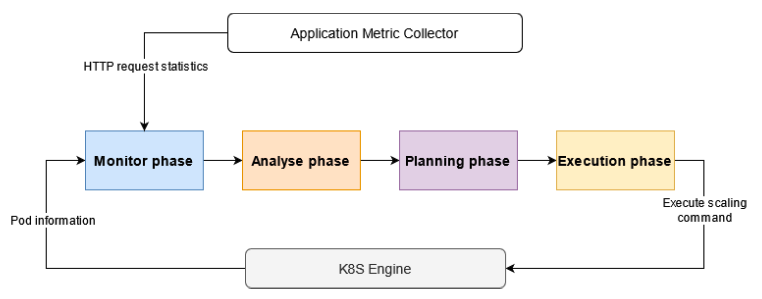
\includegraphics[width=0.8\textwidth]{chapter-2/mape.png}
    \caption{Arsitektur Sistem MAPE, \parencite{riset1}}
    \label{fig:mape}
\end{figure}

Riset ini melakukan perbandingan terhadap model ARIMA dan LSTM. Secara keseluruhan, hasil eksperimen dengan beberapa data set seperti \textit{The FIFA World Cup} dan \textit{NASA} yang berisikan logs web dari instansi terkait. Ditemukan bahwa error ketiga model ini (Bi-LSTM, ARIMA, dan LSTM) tidak signifikan. Meskipun begitu, Bi-LSTM memiliki kecepatan dan akurasi yang sangat baik dibanding kedua model lainnya. Namun, tentu saja ini bergantung pada konfigurasi model Bi-LSTM serta algoritma pada fase analisa. Sedangkan untuk uji kompleksitas, ARIMA sangat unggul karena sederhana dan tidak memerlukan banyak percobaan terhadap konfigurasi serta algoritma.

\subsection{\textit{Adaptive Scaling of Kubernetes Pods}}

\subsection{Penelitian Lainnya}

Adapun \textit{autoscaler} yang sudah dikembangkan dan dibahas di banyak penelitian lain. Pendekatan dan metode yang digunakan sangat variatif. Gambaran umum mengenai penelitian lain yang berhubungan dengan \textit{autoscaler} menggunakan model prediksi, \textit{treshold} atau \textit{rule based} maupun \textit{machine learning} bisa dilihat pada tabel.

\begin{longtable}{|p{2in}|c|p{1in}|c|p{0.8in}|}

    \caption{Tabel Penelitian Lain terkait Pengembangan Metode \textit{Autoscaling}} \label{tab:overview-autoscaler} \\

    \hline
    \multicolumn{1}{|c|}{\textbf{Paper}} & \textbf{Virtualisasi} & \multicolumn{1}{|c|}{\textbf{Metrik}} & \textbf{Pendekatan} & \multicolumn{1}{|c|}{\textbf{Metode}} \\
    \hline
    \endfirsthead
    %
    \endhead
    %
    \textit{Intelligent Workload Factoring for a Hybrid Cloud Computing Model}, \parencite{zhang} & VM & \textit{Request Rate} & Reaktif & ARIMA \tabularnewline

    \textit{Autonomic Vertical Elasticity of Docker Containers with Elasticdocker}, \parencite{al2017autonomic} & \textit{Container} & Prosesor, Memori & Reaktif & \textit{Rule-based} \tabularnewline

    \textit{Horizontal Pod Autoscaler}, \parencite{hpa2} & \textit{Container} & Prosesor & Reaktif & \textit{Rule-based} \tabularnewline

    \textit{A Novel Resource Prediction and Provisioning Scheme in Cloud Data Center}, \parencite{rpps} & \textit{Container} & Prosesor & Proaktif & ARMA \tabularnewline

    \textit{Workload Prediction Using ARIMA Model and Its Impact on Cloud Applications QoS}, \parencite{workloadprediction} & VM & \textit{Request Rate} & Proaktif & ARIMA \tabularnewline

    \textit{Resource Elasticity Controller for Docker-based Web Applications}, \parencite{resourceelasticity} & \textit{Container} & \textit{Request Rate} & Proaktif & ARIMA \tabularnewline

    \textit{Combining Time Series Prediction Models using Genetic Algorithm to Autoscaling Web Applications Hosted in the Cloud Infrastructure}, \parencite{tspwithga} & - & \textit{Request Rate} & Proaktif & \textit{Genetic Algorithm} \tabularnewline

    \textit{Predicting Cloud Resource Provisioning using Machine Learning Techniques}, \parencite{predictcloudrsrc} & - & \textit{Task Length} & Proaktif & \textit{Artificial Neural Network} \tabularnewline

    \textit{Auto-scaling Microservices on IaaS under SLA with Cost-Effective Framework}, \parencite{asmicrocosteff} & VM & \textit{Request Rate} & Proaktif & \textit{Artificial Neural Network}, \textit{Recurrent Neural Network} \tabularnewline

    \textit{Machine Learning-based Auto-scaling for Containerized Applications}, \parencite{mlbasconapps} & \textit{Container} & \textit{Request Rate} & Proaktif & LSTM \tabularnewline

    \textit{Adaptive Horizontal Scaling of Microservices using Bi-LSTM}, \parencite{adaptivehsmicro} & \textit{Container} & Prosesor, Memori & Gabungan & Bi-LSTM \tabularnewline

    \hline
\end{longtable}